\begin{markdown}
#30天 LaTeX 挑戰 Day 23 pgfplots

-----

###折線圖

除了函數圖外,pgfplots 也可以繪製折線圖。

```latex
\begin{tikzpicture}
\begin{axis}
\addplot coordinates{(0,0)(1,4)(2,3)(3,5)(4,2)(5,1)(6,0)(7,8)};
\end{axis}
\end{tikzpicture}
```

在 coordinates 後面的將放入所有折線圖的點,就可以畫出折線圖了,但有時座標軸上的標記與想像中的並不一樣,這時就需要用 xtick 與 ytick 調整。

```latex
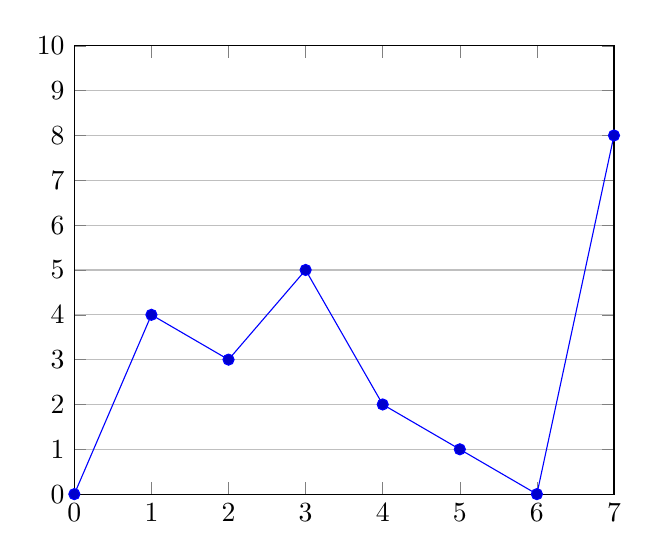
\begin{tikzpicture}
\begin{axis}[
xmin=0, xmax=7,
ymin=0, ymax=10,
xtick={0,1,2,3,4,5,6,7},
ytick={0,1,2,3,4,5,6,7,8,9,10},
ymajorgrids=true,
]
\addplot coordinates{(0,0)(1,4)(2,3)(3,5)(4,2)(5,1)(6,0)(7,8)};
\end{axis}
\end{tikzpicture}
```

* xmin, ymin, xmax, ymax 這些是指定 x 軸與 y 軸的最大、最小值
* xtick, ytick 是指定 x 軸與 y 軸上的標記的位置
* ymajorgrids 是繪製出與 y 軸相交的格線,可以用 xmajorgrids 來繪製出與 x 軸相交的格線,或用 grids=major 同時繪製兩者。

###長條圖

長條圖與折線圖有者異曲同工之妙

```latex
\begin{tikzpicture}
\begin{axis}[ybar, ybar interval=0.75, enlargelimits=0.1]
\addplot coordinates{(2040,9.50)(2030,10.60) (2020,12.58)};
\addplot coordinates{(2020,17.50) (2030,24.10) (2040,30.60)};
\legend{0~14歲人口所占比率(\%),65歲以上人口所占比率(\%)}
\end{axis}
\end{tikzpicture}
```

* ybar 指的是長條與 y 軸平行,另外還有 xbar 這個選項可以用。
* ybar interval 是指定長條之間的空隙,1 代表沒有空隙。
* enlarge limits 是調整整個座標軸與圖表的元素間的距離,另外也可以用enlarge x limits, enlarge y limits 等等來單獨調整特定的座標軸。

###散佈圖

散佈圖也很簡單。

```latex
\begin{tikzpicture}
\begin{axis}
\addplot[scatter, mark=*, only marks]
coordinates{(143,62) (50,594) (165,53) (139,348) (145,194) (75,533) (51,258) (154,492)};
\end{axis}
\end{tikzpicture}
```

* scatter 是讓顏色依據 y 軸的數值而變化
* only marks 是不讓點之間用線連起來
* mark 是指定點的標記的樣式

###從其他檔案輸入數據

上面的方法這只適用於數據只有寥寥幾筆時,不然如果有一千多筆,一個一個 key 未免太過勞神費力,不過 pgfplots 都幫你想好了,他可以讓你從 .dat 或 .csv 檔中輸入數據。

```latex
\begin{tikzpicture}
\begin{axis}[x tick label style={/pgf/number format/1000 sep=},width=10cm, grid=major]
\addplot table [x=year, y=youth, col sep=comma, mark=none] {data.csv};
\addlegendentry{0~14歲人口所占比率(\%)}
\addplot table [x=year, y=old, col sep=comma, mark=none] {data.csv};
\addlegendentry{65歲以上人口所占比率(\%)}
%\addplot table[meta=mid]{output.dat};
\end{axis}
\end{tikzpicture}
```

* x tick label style 是調整 x 軸上標示的樣式。
* table 是表示資料來源是類似表格的形式。
* x=, y= 是指定 x, y 的數據要從哪一欄輸入。
* col sep 是告訴 pgfplots 欄與欄的分界是用什麼符號。

##三維圖形

終於進入三維圖形了,

\end{markdown}